
%% This is file `elsarticle-template-1-num.tex',
%%
%% Copyright 2009 Elsevier Ltd
%%
%% This file is part of the 'Elsarticle Bundle'.
%% ---------------------------------------------
%%
%% It may be distributed under the conditions of the LaTeX Project Public
%% License, either version 1.2 of this license or (at your option) any
%% later version.  The latest version of this license is in
%%    http://www.latex-project.org/lppl.txt
%% and version 1.2 or later is part of all distributions of LaTeX
%% version 1999/12/01 or later.
%%
%% Template article for Elsevier's document class `elsarticle'
%% with numbered style bibliographic references
%%
%% $Id: elsarticle-template-1-num.tex 149 2009-10-08 05:01:15Z rishi $
%% $URL: http://lenova.river-valley.com/svn/elsbst/trunk/elsarticle-template-1-num.tex $
%%
\documentclass[preprint,12pt]{elsarticle}

%% Use the option review to obtain double line spacing
%% \documentclass[preprint,review,12pt]{elsarticle}

%% Use the options 1p,twocolumn; 3p; 3p,twocolumn; 5p; or 5p,twocolumn
%% for a journal layout:
%% \documentclass[final,1p,times]{elsarticle}
%% \documentclass[final,1p,times,twocolumn]{elsarticle}
%% \documentclass[final,3p,times]{elsarticle}
%% \documentclass[final,3p,times,twocolumn]{elsarticle}
%% \documentclass[final,5p,times]{elsarticle}
%% \documentclass[final,5p,times,twocolumn]{elsarticle}

%% The graphicx package provides the includegraphics command.
\usepackage{graphicx}
%% The amssymb package provides various useful mathematical symbols
\usepackage{amssymb}
%% The amsthm package provides extended theorem environments
%% \usepackage{amsthm}

%% The lineno packages adds line numbers. Start line numbering with
%% \begin{linenumbers}, end it with \end{linenumbers}. Or switch it on
%% for the whole article with \linenumbers after \end{frontmatter}.
\usepackage{lineno}
\usepackage{mathtools}
%% natbib.sty is loaded by default. However, natbib options can be
%% provided with \biboptions{...} command. Following options are
%% valid:

%%   round  -  round parentheses are used (default)
%%   square -  square brackets are used   [option]
%%   curly  -  curly braces are used      {option}
%%   angle  -  angle brackets are used    <option>
%%   semicolon  -  multiple citations separated by semi-colon
%%   colon  - same as semicolon, an earlier confusion
%%   comma  -  separated by comma
%%   numbers-  selects numerical citations
%%   super  -  numerical citations as superscripts
%%   sort   -  sorts multiple citations according to order in ref. list
%%   sort&compress   -  like sort, but also compresses numerical citations
%%   compress - compresses without sorting
%%
%% \biboptions{comma,round}

% \biboptions{}

\journal{Comunicaciones inal\'ambricas}

\begin{document}

\begin{frontmatter}

%% Title, authors and addresses

\title{Pr\'actico Comunicaciones Inal\'ambricas -- punto 1}

%% use the tnoteref command within \title for footnotes;
%% use the tnotetext command for the associated footnote;
%% use the fnref command within \author or \address for footnotes;
%% use the fntext command for the associated footnote;
%% use the corref command within \author for corresponding author footnotes;
%% use the cortext command for the associated footnote;
%% use the ead command for the email address,
%% and the form \ead[url] for the home page:
%%
%% \title{Title\tnoteref{label1}}
%% \tnotetext[label1]{}
%% \author{Name\corref{cor1}\fnref{label2}}
%% \ead{email address}
%% \ead[url]{home page}
%% \fntext[label2]{}
%% \cortext[cor1]{}
%% \address{Address\fnref{label3}}
%% \fntext[label3]{}


%% use optional labels to link authors explicitly to addresses:
%% \author[label1,label2]{<author name>}
%% \address[label1]{<address>}
%% \address[label2]{<address>}

\author{Santiago Nolasco}

\address{FI, IUA}


\begin{keyword}
XBee \sep Path loss \sep Friis
%% keywords here, in the form: keyword \sep keyword

%% MSC codes here, in the form: \MSC code \sep code
%% or \MSC[2008] code \sep code (2000 is the default)

\end{keyword}

\end{frontmatter}

%%
%% Start line numbering here if you want
%%
%\linenumbers

%% main text
\section{C\'alculo de enlace y modelos de propagaci\'on}
\label{S:1}

Maecenas \cite{Smith:2012qr} fermentum \cite{Smith:2013jd} urna.

El dise\~no de un radioenlace implica toda una serie de c\'alculos que pueden resultar sencillos o complicados, dependiendo de las caract\'eristicas del sistema y del tipo de problema al que nos enfrentemos.

Es por ello que podemos dividir la propagaci\'on de la se\~nal de acuerdo al entorno donde esta viaje: 

\begin{itemize}
\item Espacios abiertos 
\item Entornos cerrados
\end{itemize}


\subsection{Distancia m\'axima en espacios abiertos}

 La comunicaci\'on "outdoor" en este problema se asume en un entorno de propagaci\'on libre, donde no existen p\'erdidas atmosf\'ericas, de polarizaci\'on y de desadaptaci\'on de impedancias, es decir, operamos en regiones descubiertas. 
 
\begin{figure}[h]
	%\DeclareGraphicsExtensions{.pdf,.png,.jpg,.ppm}
	\centering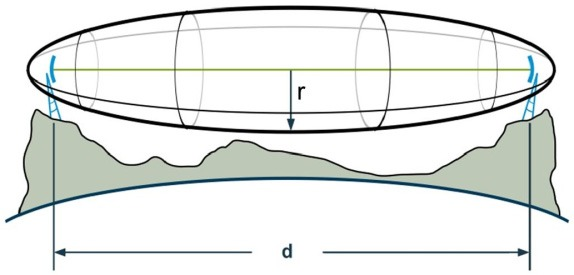
\includegraphics[width=0.8\linewidth]{Image}
	\caption{Primer zona de Fresnel}
\end{figure}

\begin{table}[h]
\centering
\begin{tabular}{l l l}
\hline
\textbf{Modo de funcionamiento} & \textbf{Normal} & \textbf{Boost}\\
\hline
Potencia de Tx & +5dBm(3.1mW) & +8dBm(6.3mW) \\
Sensibilidad de Rx & -100dBm & -102dBm\\
\hline
\end{tabular}
\caption{Technical review Xbee ZB}
\end{table}
Para los c\'alculos siguientes se tomar\'an los datos de funcionamiento en modo "Normal".

Partiendo de la ecuaci\'on de Friis

%\begin{equation}
%\label{Ecuaci\'on de Friis}

%Pr = \frac{Pt Gt Gr \lambda ^{2}}{(4\pi R)^2}

%\end{equation}

\begin{equation*}
\label{Ec:Friis}
Pr = \frac{Pt Gt Gr \lambda ^{2}}{(4\pi d)^2}
\end{equation*}
Siendo Pr (Potencia recibida), Pt(Potencia transmitida), Gt(Ganancia de antena tx), Gr(Ganancia de antena rx), $\lambda$(longitud de onda) y d(distancia radial entre antenas).

Podemos despejar la atenuaci\'on de espacio libre, tambi\'en conocida como p\'erdida de trayectoria.
\begin{equation*}
\label{Ec:perdida}
P_{Loss}[dB] = 94.4 + 20 \log_{10}d [Km] + 20 \log_{10}f [GHz] - Gt[dBi] - Gr[dBi]
\end{equation*}
	Y de esta despejar la m\'axima distancia
\begin{equation*}
\label{Ec:distancia}
d[Km] = 10^{\frac{P_{Loss} + Gt + Gr - 20 \log_{10}f - 92.4}{20}}
\end{equation*}
$P_{Loss}=Gt[dBm] - Gr[dBm] = +5dBm - (-100dBm) = 105dBm$
$f = 2.4 [GHz]$
Las ganancias Gr[dBi] y Gr[dBi] se toman como valor cero por ser antenas omnidireccionales.
\begin{equation*}
\label{Ec:distancia1}
d[Km] = 10^{\frac{105 dBm - 20 \log_{10}2.4 - 92.4}{20}} = 1.77 [Km] =1770m
\end{equation*}	
Con la m\'axima distancia $d$ del radioenlace, calculamos la altura $r$ de las antenas. Para ello nos valemos de las f\'ormulas del primer elipsoide de Fresnel, esto es determinando la zona libre de obstaculos.
\begin{equation*}
\label{Ec:fresnel}
r = F1(m) = 17.32 \sqrt{\frac{(d[Km]/2)^2}{d[Km]f[GHz]}} = 17.32 \sqrt{\frac{(1.77Km/2)^2}{1.77Km2.4GHz}} = 7.43m
\end{equation*}	

Por lo tanto la altura de las antenas, es decir para establecer una comunicaci\'on punto a punto a distancia m\'axima $d=1.77Km$ entre 2 XBee es de $r=7.43$ en la zona libre de obstaculos.

\subsection{Distancia m\'axima en entornos cerrados}

La propagaci\'on "indoor" difiere respectos a los sistemas "outdoor". Para asegurar una eficiente comunicaci\'on interior, la ITU a llevado una serie de propuestas para el caso de comunicaciones punto a punto. Debido a que en una comunicaci\'on en entornos cerrados esta muy influenciada por la geometr\'ia del lugar y los objetos en ella. Tanto estos objetos y la construcci\'on de la misma, ocasionan p\'erdidas por reflexiones, dispersi\'on y absorci\'on de las se\~nales RF.  

\begin{figure}[h]
%\centering\includegraphics[width=0.4\linewidth]{placeholder}
\caption{Figure caption}
\end{figure}

\subsubsection{C\'alculo Planta alta}
Para el c\'alculo de m\'axima distancia, como lo indica la figura. Nos valdremos de la f\'ormula de "path loss"
\begin{equation*}
\label{eq:pathLoss}
L_{Loss}[dB] = L_{do}[dB] + N \log_{10}d/do + Lf_{n}[dB]
\end{equation*}
Donde $N$(Coef. de p\'erdida), $f$(Frecuencia en Mhz),$d$(Distancia entre base y terminal), $L_{do}$(P\'erdida a do), $L_{f}$(Atenuaci\'on trav\'es del piso), $d0$(distancia de ref=1m) y $n$(nro de pisos entre terminal y base).
En nuestro caso particular al igual que en el caso anterior, calculamos la m\'axima atenuaci\'on:
$L_{Loss}= Gt - Gr = +5dBm - (-100dBm) = 105dBm$
$N=28$ Por dato de tabla (Espacio residencial a 2.4GHz).
$L_{do} = 20 \log_{10}f[MHz] - 28 = 39.6dB$
$Lf_{n} = 0$ Por ser un mismo piso.
Despejando d
\begin{equation*}
\label{eq:calculod}
d[m] = 10 ^{\frac{L_{Loss}[dB] - L_{do}[dB] - L_{f}[dB]}{N}} 
d[m] = 10 ^{\frac{105dBm - 39.6dB - 0}{28}} = 216.62m
\end{equation*}
Entonces en un piso la distancia m\'axima de transmisi\'on es $d=216.62m$

\subsubsection{C\'alculo de comunicaci\'on entre Planta alta y baja}
En este caso la m\'axima distancia $d$, ser\'a influenciada por la atenuaci\'on del piso, como separaci''on de los dos ambientes. Por lo tanto $L_{f}[dB]=5$ dado por el cuadro. La distancia m\'axima ser\'a.
\begin{equation*}
\label{eq:calculod}
d[m] = 10 ^{\frac{L_{Loss}[dB] - L_{do}[dB] - L_{f}[dB]}{N}} 
d[m] = 10 ^{\frac{105dBm - 39.6dB - 5}{28}} = 143.59m
\end{equation*}
Se puede notar aqu\'i, que el valor de $d$ distancia m\'axima es reducido por esta atenuaci\'on. Siendo el valor de $d=143.59m$ para comunicaciones entre dos pisos.
%% The Appendices part is started with the command \appendix;
%% appendix sections are then done as normal sections
%% \appendix

%% \section{}
%% \label{}

%% References
%%
%% Following citation commands can be used in the body text:
%% Usage of \cite is as follows:
%%   \cite{key}          ==>>  [#]
%%   \cite[chap. 2]{key} ==>>  [#, chap. 2]
%%   \citet{key}         ==>>  Author [#]

%% References with bibTeX database:

\bibliographystyle{model1-num-names}
\bibliography{sample.bib}

%% Authors are advised to submit their bibtex database files. They are
%% requested to list a bibtex style file in the manuscript if they do
%% not want to use model1-num-names.bst.

%% References without bibTeX database:

% \begin{thebibliography}{00}

%% \bibitem must have the following form:
%%   \bibitem{key}...
%%

% \bibitem{}

% \end{thebibliography}


\end{document}

%%
%% End of file `elsarticle-template-1-num.tex'.
              